%\newcommand{\eps}{\epsilon}
\newcommand{\Pmax}{p_\text{max}} 	
\newcommand{\Hint}{H_{int}}
\newcommand{\kbar}{\bar{k}}
\newcommand{\Delk}{\Delta}
\newcommand{\Sumk}{\Sigma}
\newcommand{\Qrot}{Q_{pq}(\tau_s)}
\newcommand{\shapecor}{\mathcal{S}}
\newcommand{\ampcor}{\mathcal{A}}
\newcommand{\totalcor}{\mathcal{E}}
\newcommand{\threeLs}{L_p(\kbar_1)L_q(\kbar_2)L_r(\kbar_3)}
\newcommand{\threePs}{P_p(\kbar_1)P_q(\kbar_2)P_r(\kbar_3)}
\newcommand{\threeQs}{Q_p(k_1)Q_q(k_2)Q_r(k_3)}
\newcommand{\Lbasic}{\mathcal{P}_0}
\newcommand{\Linvk}{\mathcal{P}_1}
\newcommand{\Lnsinv}{\mathcal{P}^{n_s}_1}
\newcommand{\Lnsboth}{\mathcal{P}^{n_s}_{01}}
\newcommand{\Linvksq}{\mathcal{P}_2}
\newcommand{\Lns}{\mathcal{P}^{n_s}_2}
\newcommand{\Fbasic}{\mathcal{F}_0}
\newcommand{\Finvk}{\mathcal{F}_1}
\newcommand{\Finvksq}{\mathcal{F}_2}
\newcommand{\quadpot}{V_{\phi^2}(\phi)}
%\newcommand{\threeqs}{q_p(\kbar_1)\,q_r(\kbar_2)\,q_s(\kbar_3)}
\newcommand{\threeqs}{q_p(k_1)\,q_r(k_2)\,q_s(k_3)}
\newcommand{\threeqstilde}{q_{\tilde{p}}(k_1)\,q_{\tilde{r}}(k_2)\,q_{\tilde{s}}(k_3)}
\newcommand{\kmin}{{k_\text{min}}}
\newcommand{\kmax}{{k_\text{max}}}
\newcommand{\fnl}{f_{NL}}
\newcommand{\fnllocal}{f^{local}_{NL}}
\newcommand{\fnlequil}{f^{equil}_{NL}}
\newcommand{\fnlortho}{f^{ortho}_{NL}}

\chapter{An Inflationary Constraint from the $\cmb$ Bispectrum}\label{chapter:constraints}
\section{The $\primodal$-$\cmbbest$ pipeline}
    In this chapter, we aim to validate our full pipeline,
    testing the connection between the methods we described in previous Chapters~\ref{chapter:decomp}
    and~\ref{chapter:methods}
    (implemented in the $\primodal$ code) and the methods described in~\cite{Sohn_2021}
    (which are implemented in the $\cmbbest$ code, which we discussed
    in Section~\ref{sec:cmbbest}).
    We perform this validation by
    using $\planck$ data to place a constraint on the sound speed in $\dbi$ inflation~\eqref{eq:dbi_action}.
    We then compare this result to a constraint on the same parameter obtained by the $\planck$
    collaboration~\cite{Planck_NG_2018}.


    %with the aim of validating the full $\primodal$-$\cmbbest$ pipeline.
    The $\planck$ result~\cite{Planck_NG_2018} was obtained by constraining the amplitude
    of the $\dbi$ template~\eqref{dbi_shape}, and using the relation~\eqref{fnl_dbi_defn}
    to map this to a constraint on the sound speed.
    In our pipeline, in contrast, we scan over a parameter of the model, $\bir$~\eqref{eq:dbi_warp},
    with the other parameters of the model held fixed.
    This means the sound speed of a given scenario is not a constant, and is instead found by numerically evolving the background.
    We use $c_s^*$ to refer to the sound speed (of each scenario) at horizon crossing of the pivot scale.
    We obtain the full shape and amplitude information (within our $k$-range) for
    each scenario in our scan and the final
    constraint makes use of the entirety of that information, up to
    convergence in $\Pmax$, the size of the basis.


    One important limitation of our scan, however, is that we do not
    prescribe how inflation ends, as we neglect the details of reheating.
    This means that we do not have a mapping from the scales during inflation and the observable scales
    today. As such, the constraint we obtain on the sound speed during inflation
    cannot be directly translated into a constraint on more fundamental parameters
    (as was done, for example, in~\cite{Planck_NG_2013} where the sound speed constraint
    was translated into a constraint on a fundamental parameter by marginalising over the
    number of inflationary e-folds).
    Our result is still a useful validation of our pipeline---specifically, we validate the
    accuracy and convergence (in $\Pmax$)
    of our methods at the level of the constraint, demonstrating that this pipeline can be applied to constraining
    inflationary parameters, and can handle bispectra that are non-separable and include
    slow-roll corrections such as a non-separable scaling.


    In the context of the scan
    (which we will describe in Section~\ref{sec:setup}),
    we used the methods described in previous chapters (as implemented in
    the $\primodal$ code) to generate shape coefficients for each scenario in the scan.
    The $\cmbbest$ code, which implements the methods described in~\cite{Sohn_2021},
    then used the $\planck$ 2018 temperature\footnote{
        At present the $\cmbbest$ code is implemented for temperature only, but the methods are general
        and future implementations will include E-mode polarisation.
    } data to place a constraint
    on $c_s^*$.


    We can gain some context on the expected method variance of bispectrum estimators by simply examining the
    scatter between the estimators used within the $\planck$ 2018 analysis.
    Note that this is not statistical variance, but simply method variance,
    coming from the difficulty of $\cmb$ bispectrum estimation.
    We show this in Figure~\ref{fig:equil_constraints_comparison} for the equilateral template~\eqref{equil_shape}
    which is closely related to the $\dbi$ template.
    We see that the result obtained by $\cmbbest$ is different, but still lies
    between the results of the $\ksw$ and $\modal$ estimators.
    For a discussion on the scatter between the estimators used in the $\planck$ analysis,
    see Appendix B of~\cite{Planck_NG_2013}. In that work it was concluded that in ideal conditions
    (no noise, no sky mask) the scatter between estimators would be entirely due to their respective
    approximations of the primordial shapes, with the approximations being such that a scatter
    of $0.3\sigma$ would be expected.


    \begin{figure}[h!]
        \centering
        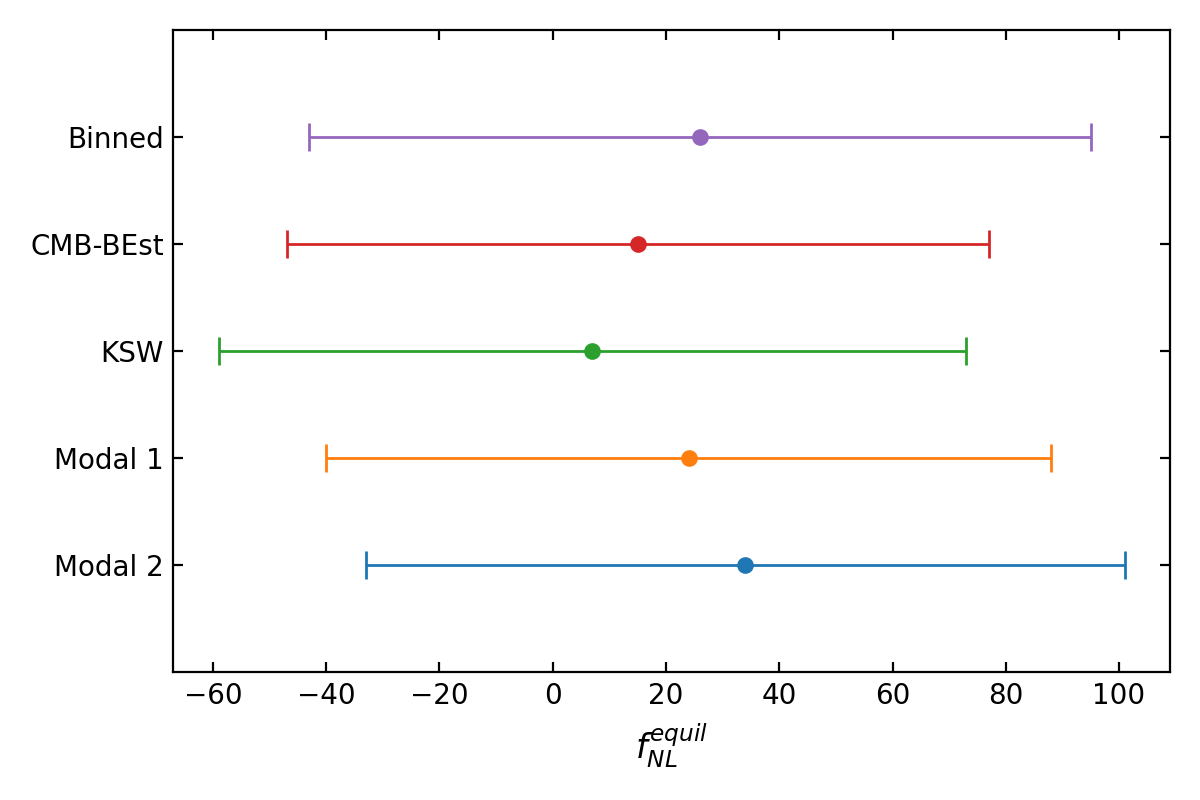
\includegraphics[width=0.9\textwidth]{wuhyun_plots/fnl_equil_planck_scatter.png}
        \caption{
            A comparison of the various estimation methods used in $\planck$,
            as presented in table 5 of~\cite{Planck_NG_2018},
            with the $\cmbbest$ result, presented in~\cite{Sohn_2021}.
            We plot the constraints obtained by each method for $\fnlequil$,
            along with their $68\%$ uncertainty margin.
            Note that the estimation methods are optimal
            (at least to a very good approximation),
            hence their uncertainty margins are close to identical.
            We see that while the estimators do not agree, there is no discrepancy with any
            significance---in particular, we see that $\cmbbest$ is not an outlier.
            %Possible contributions to the difference in the central values are convergence in each
            %method (for their respective convergence parameters)
            %and numerical issues.
            %It is important to note that the differences between the
            %different results are not due to statistical variance.
            The $\cmbbest$ result quoted here was obtained by decomposing the equilateral
            template~\eqref{equil_shape} (using definition~\eqref{planck_fnl_defn_ns} for $\fnlequil$)
            in the $\Lnsinv$ basis for $\Pmax=30$.
        }\label{fig:equil_constraints_comparison}
    \end{figure}


    In our pipeline,
    the bispectrum of each scenario is given an amplitude
    parameter which we call $\fnlone$, where the scenario prediction
    corresponds to $\fnlone=1$ (schematically $\alpha_{pqr}\rightarrow\fnlone \alpha_{pqr}$).
    Thus, if we find that $\fnlone=1$ is inconsistent with the data,
    we can judge that scenario to be inconsistent with the data as well.
    The $\cmbbest$ code determines the confidence interval of the result
    by applying the estimator to $140$ full focal plane realistic Gaussian
    simulations~\cite{Planck_ffp10_2015}. The variance of the results from those
    Gaussian maps is then assumed to approximate the variance of the result
    when the estimator is applied to a $\cmb$ drawn from a universe with $\fnlone=1$,
    motivated by the expectation that the non-Gaussianity is weak.


\section{Scan parameters}\label{sec:setup}
The potential we use is the IR one discussed in~\cite{Bean_ir_dbi}, as
we outlined in Section~\ref{sec:interactions}.
See also~\cite{Chen_dbi, warp_features_dbi} for further discussions.
    We use equation~\eqref{eq:dbi_warp}, which has four free parameters,
    $\bir$, $\lambda_{\dbi}$, $\phi_0$, and $V_0$.
    We use $\bir$ to parameterise our scan,
    which we take across the range
    \begin{align}\label{eq:bir_range}
        %\bir\in[0.1885, 0.58].
        \bir\in[0.19, 0.58].
    \end{align}
    with the parameters
    \begin{align}\label{eq:scan_params}
        \lambda_{\dbi}&=2.00475\times10^{15}\\
        V_0 &= 5.2\times10^{-12}\mpl^4\\
        \phi_0 &= 0.46042\mpl
    \end{align}
    held fixed.
    This will give an approximately fixed power spectrum, with a realistic
    scaling ($n_s^{*}$ is within $0.9649\pm0.0042$ across the scan),
    while allowing the bispectrum to vary across the scan.


    The number of e-folds to the end of inflation is denoted $N_e$.
    From~\cite{Chen_dbi} we can use slow-roll relations to determine the approximate
    value of $N_e$
    %We find
    for our values of $\phi$ as
    \begin{align}
        N_e &= \frac{\sqrt{\lambda_{\dbi}}H}{\phi}\approx10^2.%112
    \end{align}
    We can also then write down the expected relation between the sound speed
    and $\bir$
    \begin{align}
        c_s &\approx \frac{3}{\bir N_e}%&&\approx 0.054.
    \end{align}
    which we indeed find to be approximately true for our numerical results.
    We start the background evolution on the slow-roll attractor, finding initial conditions which
    satisfy the Friedmann constraint, as discussed in Section~\ref{sec:interactions}.
    %For each scenario in this scan we ensure that $\ln\left(10^{10}A_s\right)$
    %is within $3.044\pm0.014$,
    %and that $n_s^{*}$ is within $0.9649\pm0.0042$.
    In Table~\ref{tab:scan_summary_sr} we summarise the scenario parameters for the scan,
    and in Table~\ref{tab:scan_summary_ns} we summarise the resulting scaling indices.
 

%    \begin{tabular}{lrrrrrrrrrr}
%        \toprule
%        $\bir$ &    $c_s^{*}$ &  $\varepsilon_s^{*}$ &   $\varepsilon^{*}$ &   $n_s^{*}$ &  $n_{NG}^{*}$ &   $\phi^{*}$ &     $H^{*}$ &   $\eta^{*}$ \\
%        \midrule
%        $1.89\times 10^{-1}$  &  $1.39\times 10^{-1}$  &  $  8.57\times 10^{-3}$  &  $7.44\times 10^{-5}$  &  $-3.50\times 10^{-2}$  &  $-8.72\times 10^{-2}$  &  $5.19\times 10^{-1}$  &  $1.31\times 10^{-6}$  &  $2.63\times 10^{-2}$ \\
%        $5.80\times 10^{-1}$  &  $4.50\times 10^{-2}$  &  $  8.67\times 10^{-3}$  &  $2.31\times 10^{-4}$  &  $-3.63\times 10^{-2}$  &  $-8.99\times 10^{-2}$  &  $5.15\times 10^{-1}$  &  $1.30\times 10^{-6}$  &  $2.71\times 10^{-2}$ \\
%        \bottomrule
%    \end{tabular}
    %in Table~\ref{tab:scan_summary_bkgd} we summarise the background parameters,

\begin{table}[h!]
  \begin{center}
    \begin{tabular}{lrrr}
        \toprule
        $\bir$ &    $c_s^{*}$ &  $\varepsilon_s^{*}$ &   $\varepsilon^{*}$ \\
        \midrule
        $1.89\times 10^{-1}$  &  $1.39\times 10^{-1}$  &  $  8.57\times 10^{-3}$  &  $7.44\times 10^{-5}$  \\
        $5.80\times 10^{-1}$  &  $4.50\times 10^{-2}$  &  $  8.67\times 10^{-3}$  &  $2.31\times 10^{-4}$  \\
        \bottomrule
        $\bir$ &    $\eta^{*}$ &  $\phi^{*}~[\mpl]$ &     $H^{*}~[\mpl]$ \\
        \midrule
        $1.89\times 10^{-1}$  &  $2.63\times 10^{-2}$ &  $5.19\times 10^{-1}$  &  $1.31\times 10^{-6}$\\
        $5.80\times 10^{-1}$  &  $2.71\times 10^{-2}$ &  $5.15\times 10^{-1}$  &  $1.30\times 10^{-6}$\\
        \bottomrule
    \end{tabular}
    \caption{
        Summary of scenario parameters at the upper and lower limits of the scan, evaluated at the horizon
      crossing of the pivot scale.
      }\label{tab:scan_summary_sr}
  \end{center}
\end{table}


%\begin{table}[h!]
%  \begin{center}
%    \begin{tabular}{lrrr}
%        \toprule
%        $\bir$ &  $\phi^{*}$ &     $H^{*}$ \\
%        \midrule
%        $1.89\times 10^{-1}$  &  $5.19\times 10^{-1}$  &  $1.31\times 10^{-6}$\\
%        $5.80\times 10^{-1}$  &  $5.15\times 10^{-1}$  &  $1.30\times 10^{-6}$\\
%        \bottomrule
%    \end{tabular}
%    \caption{Summary of scenario parameters across the scan.}\label{tab:scan_summary_bkgd}
%  \end{center}
%\end{table}


\begin{table}[h!]
  \begin{center}
    \begin{tabular}{lrr}
        \toprule
        $\bir$ &  $n_s^{*}$ &  $n_{NG}^{*}$\\
        \midrule
        $1.89\times 10^{-1}$  &  $9.650\times 10^{-1}$  &  $-8.72\times 10^{-2}$\\
        $5.80\times 10^{-1}$  &  $9.637\times 10^{-1}$  &  $-8.99\times 10^{-2}$\\
        \bottomrule
    \end{tabular}
      \caption{
          Summary of the slow-roll predictions for the scaling indices
          at the upper and lower limits of the scan.
      }\label{tab:scan_summary_ns}
  \end{center}
\end{table}


\section{$\dbi$ sound speed constraint}
    At present $\cmbbest$ has been run for the $\Lnsinv$ basis
    with $\Pmax=30$, for the $\planck$ 2018 map and simulations~\cite{Planck_NG_2018},
    in particular the data that has been foreground cleaned using the SMICA method
    (Spectral Matching of foregrounds implementing Independent
    Component Analysis).
    To make contact with $\cmbbest$, the $\primodal$ scan
    was run with the same basis\footnote{
        The $\cmbbest$ code has also been run for a $\ksw$ basis
        and a Fourier basis, but neither of these can describe features
        with a complicated shape dependence.
        Other basis sets described in Chapter~\ref{chapter:decomp} will be used in future runs of $\cmbbest$.
    }.
    As shown in Figure~\ref{fig:dbi_sound_speed_scan_beta}, we find
    %\begin{align}\label{eq:cmbbest_bir_constraint}
    %    \bir\le0.46\qquad(95\%,~T~\text{only}).
    %\end{align}
    %This translates into
    a constraint
    on the sound speed (at horizon crossing) of
    \begin{align}\label{eq:cmbbest_dbi_constraint}
        c_s^{*}\ge0.056\qquad(95\%,~T~\text{only}).
    \end{align}


    \begin{figure}[h!]
        \centering
        %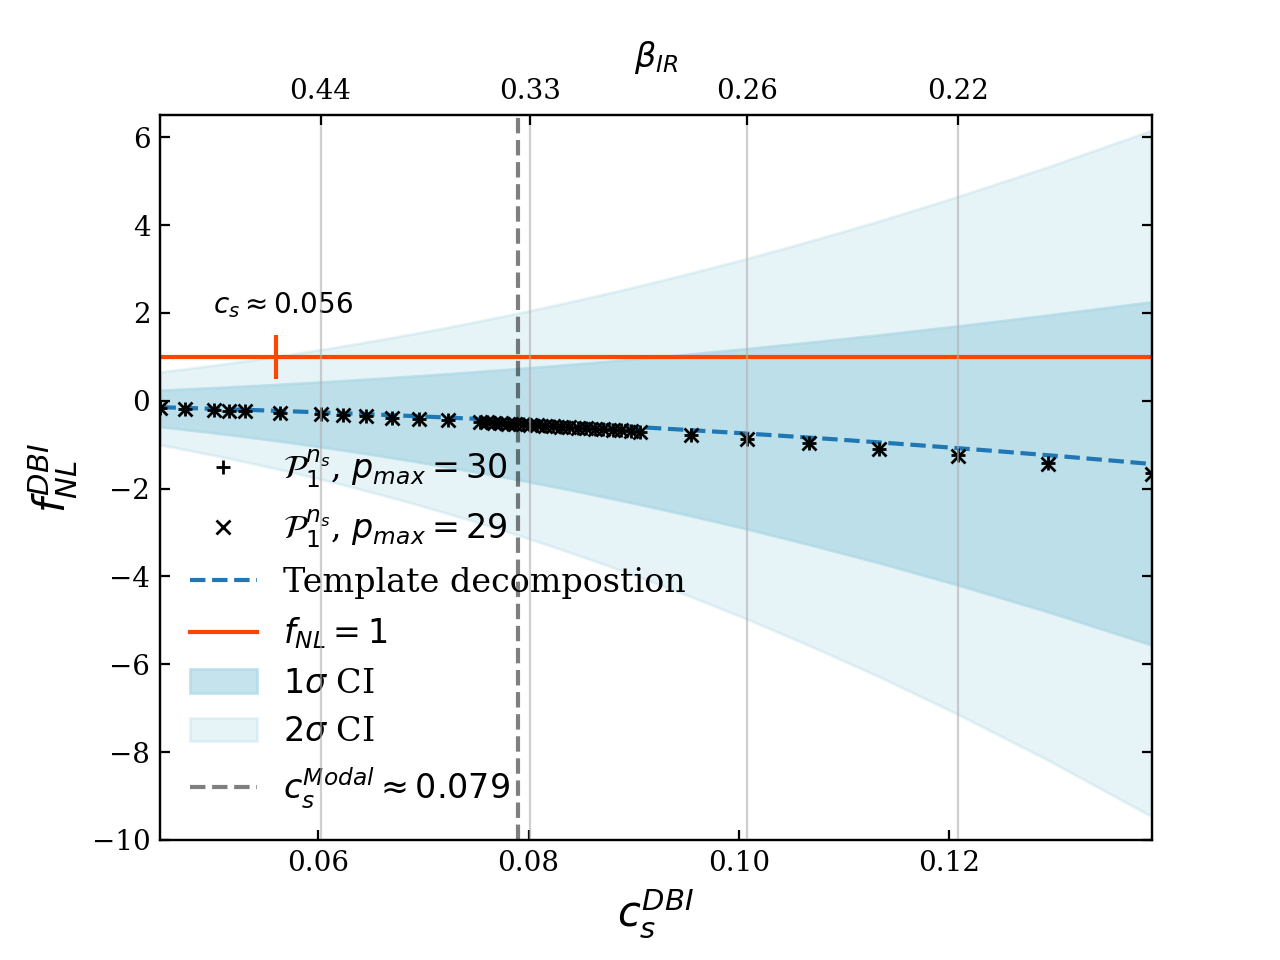
\includegraphics[width=0.9\textwidth]{wuhyun_plots/beta_ir_constraint_busy.png}
        \includegraphics[width=0.9\textwidth]{wuhyun_plots/beta_ir_constraint_with_beta.png}
        \caption{
            The constraint we obtain on $\dbi$ inflation. Here $c_s^{\dbi}$ is not an input parameter,
            unlike in the template case. Instead it is time dependent, and the value plotted as $c_s^{\dbi}$
            here is the value at horizon crossing of the pivot scale, which can be used to label the
            scenarios we scanned over.
            %We find that $\bir<0.46$
            We find $c_s^*\ge0.056$ at $95\%$ confidence.
            %0.464
            This plot was obtained by
            scanning across values of $\bir$ and calculating the corresponding primordial bispectra
            using $\primodal$, then projecting those bispectra onto the $\cmb$
            and comparing them to the $\planck$ $\cmb$ temperature data using
            $\cmbbest$. Since the amplitude is fixed by the scenario, we rule out a
            scenario by ruling out $\fnlone^{\dbi}=1$.
            %We can see that the $\cmbbest$ result does not agree with the $\modal$
            %result~\eqref{eq:planck_dbi_constraint},
            %but as we see in Figure~\ref{fig:equil_constraints_comparison},
            %the discrepancy is not unexpected. We discuss possible explanations in the text.
            Note that the $\bir$ is approximately inversely proportional to $c^*_s$.
            The confidence interval is the variance of the estimated $\fnlone$ obtained
            from $140$ Gaussian maps.
            % $\sigma$ is the expected deviation between the measured $\fnlone$ and the
            % real one? It \textit{feels} like it should be centered on zero\ldots
        }\label{fig:dbi_sound_speed_scan_beta}
    \end{figure}


    Equation (55) in~\cite{Planck_NG_2018} presents the 
    constraint on the sound speed during $\dbi$ inflation
    derived from the $\cmb$ bispectrum using the $\modal$ estimator
    \begin{align}\label{eq:planck_dbi_constraint}
        c_s^{\dbi}&\ge0.079\qquad(95\%,~T~\text{only},~\modal)
    \end{align}
    using the definition~\eqref{fnl_dbi_defn} and the template~\eqref{dbi_shape}.
    While our goal was to use this previous constraint as a validation of our own pipeline,
    it is not unexpected that we did not reproduce it exactly,
    if we recall the scatter in the estimates for $\fnlequil$
    in Figure~\ref{fig:equil_constraints_comparison}.
    One possible reason for this is the fact we are using slightly different
    scales---since we are limited to $\kmax/\kmin=1000$
    for convergence reasons, we cannot
    use all the scales in the $\planck$ data.
    %We use $\kmin=0.00020875905683771526$
    Another possible reason is convergence in the number of
    maps\footnote{
        In addition to the variance of $\fnlone$,
        the maps are used to approximate the full covariance matrix for the linear term
        (see equation~\eqref{estimator_with_linear} and discussion below)
        in the estimator of~\cite{Sohn_2021}. Thus, the estimated value of $\fnlone$
        will only converge once sufficiently many maps are used.
        However, this correction (which accounts for the effect of the mask)
        was found to typically be relevant for local-type shapes,
        and small for equilateral-type shapes, such as in $\dbi$ inflation.
    }, with $\modal$ using approximately $300$ maps while $\cmbbest$ uses $140$.
    Both of these issues would make our constraint less accurate.
    However, as we will show in~\ref{sec:dbi_convergence}, the representation of the
    shape used in the $\primodal$-$\cmbbest$ pipeline has converged to high
    precision, so we do not expect this to contribute to the discrepancy.
    %Numerical issues in either method could also contribute.
    An in-depth discussion of these possibilities will be presented in~\cite{Sohn_2021}.


\section{Convergence}\label{sec:dbi_convergence}
    It is not obvious how the convergence of the primordial bispectrum translates to
    convergence of the estimate for $\fnlone$, as different
    momentum configurations will be processed and projected differently.
    For example, if the primordial bispectrum has equal absolute error in a given
    equilateral configuration v.s.\ a squeezed configuration, will the error in
    each have comparable effect on the final constraint, or will one matter more?
    We will now discuss the convergence at the primordial level and compare it to
    the convergence in the final constraint.


    In Figure~\ref{fig:prim_conv} we show convergence results for $\Lnsinv$ with $\Pmax=30$.
    We quantify the convergence by measuring $\totalcor$, as defined in~\eqref{relative_difference}, between
    $\Pmax=30$ and $\Pmax=25$.
    For this basis the match to the template is good in the equilateral limit, but quite poor in the squeezed limit.
    The convergence in the $\scalingbasis$ basis is better, with $\totalcor$
    falling in the range $[10^{-4}, 10^{-3}]$.
    %$[1.02\times 10^{-4}, 9.24\times 10^{-4}]$.
    However, to connect to the $\cmbbest$ code we must use
    the $\Lnsinv$ basis. We see from Figure~\ref{fig:prim_conv}
    that it is sufficient for our purposes.


    In Figure~\ref{fig:cmb_conv} we see how this convergence translates to convergence
    in the final constraint, at the $\cmb$ level. We see that across the $\bir$ range,
    comparing $\Pmax=25$ and $\Pmax=30$,
    the relative error in the quantity that determines the constraint,
    $\fnlone+2\sigma$, is sufficiently small that we can be
    confident our results have converged in $\Pmax$.
    We also see that it is (for the majority of the scan) smaller
    that the corresponding relative error at the primordial level, plotted in
    Figure~\ref{fig:prim_conv}.


\begin{figure}[h!]
\centering
    \subfloat[The $\scalingbasis$ basis]{\label{fig:prim_conv_log30}
        \includegraphics[width=\columnwidth]{dbi_scan_template_corrs_plots/dbi_primodal_scan_template_corrs_log30.png}}\\
    \subfloat[The $\Lnsinv$ basis]{\label{fig:prim_conv_p1ns30}
        \includegraphics[width=\columnwidth]{dbi_scan_template_corrs_plots/dbi_primodal_scan_template_corrs_p1ns30}}\\
\caption{
    The $\scalingbasis$ basis converges well across the scan range.
    We see that the bare $\dbi$ template is a poor match to the true numerical result.
    This is mostly due to the error in the overall magnitude.
    Once this is corrected, we see that the numerical result matches the
    approximate template to better than $1\%$. As the convergence of the
    numerical result is better than $0.1\%$ for the $\scalingbasis$ basis
    we can see that sum scaling~\eqref{dbi_sum_shape} and the
    product scaling~\eqref{dbi_prod_shape} perform
    comparably in matching the numerical result. This is mostly
    due to those templates neglecting slow-roll suppressed contributions,
    which, if they have a local-type shape,
    do in fact become relevant to the primordial
    bispectrum deep enough into the squeezed limit.
    The $\Lnsinv$ basis is sufficiently convergent across the scan range
    to obtain the desired constraint.
    We see that the convergence error is only slightly better than the error
    in the slow-roll corrected templates.
    In each case we estimate the convergence at the primordial level
    by refitting the full result with $\Lnsinv$ at $\Pmax=25$, and calculating
    the relative difference $\totalcor$ between the two,
    as defined in~\eqref{relative_difference}.
}\label{fig:prim_conv}
\end{figure}


\begin{figure}[h!]
\centering
%\includegraphics[width=\columnwidth]{dbi_scan_template_corrs_plots/dbi_primodal_scan_fnl_errs_p1ns30}
\includegraphics[width=\columnwidth]{wuhyun_plots/errors_for_planck_map.png}
\caption{
    We plot the relative error in the value of $\fnlone^{2\sigma}=\fnlone+2\sigma$,
    between $\Pmax=30$ and $\Pmax=25$,
    with $\fnlone$ obtained from the $\planck$ map for each scenario in the scan.
    We see that the convergence across the majority of the scan is better than that of the
    convergence in the primordial bispectrum, as plotted in Figure~\ref{fig:prim_conv}.
    This validates the $\Pmax$ convergence of our pipeline as a whole.
}\label{fig:cmb_conv}
\end{figure}


    When we examine the convergence to the sum~\eqref{dbi_sum_shape}
    and product~\eqref{dbi_prod_shape} scaling templates,
    in Figure~\ref{fig:prim_conv},
    we see that neither is obviously the better match to the numerical result.
    This is due to the numerical result having a non-zero squeezed limit
    coming from slow-roll suppressed local-type contributions
    which are neglected in the $\dbi$ templates.


%\begin{table}[h!]
%  \begin{center}
%    \begin{tabular}{lrrrr}
%        \toprule
%        $\bir$ & Sum Template & Product Template & Bare Template & With $\Pmax=25$ \\
%        \midrule
%        $1.89\times 10^{-1}$  &  $6.15\times 10^{-3}$  &  $7.22\times 10^{-3}$  &  $5.16\times 10^{-2}$  &  $5.3\times 10^{-3}$ \\
%        $5.80\times 10^{-1}$  &  $4.51\times 10^{-3}$  &  $3.63\times 10^{-3}$  &  $5.28\times 10^{-2}$  &  $2.6\times 10^{-3}$ \\
%        \bottomrule
%    \end{tabular}
%    \caption{
%        Comparing the $\Lnsinv(\Pmax=30)$ result compared to
%        templates~\eqref{dbi_shape},~\eqref{dbi_sum_shape} and~\eqref{dbi_prod_shape}.
%        We also refit the result with $\Lnsinv(\Pmax=25)$, and compare with the full
%        result to estimate the convergence at the primordial level.
%    }\label{tab:template_errors}
%  \end{center}
%\end{table}


\section{Slow-roll effects}
    The main slow-roll corrections are a correction to the overall amplitude,
    a deviation from perfect scale-dependence,
    and a local-type contribution in the squeezed limit which eventually comes to dominate
    the primordial comoving curvature bispectrum
    for sufficiently squeezed triangles.


    We can test the impact of the slow-roll effects on the constraint by decomposing the
    $\dbi$ template~\eqref{dbi_shape} in $\Lnsinv$ and using the result
    to obtain a constraint on $c_s$.
    The constraint obtained from such a decomposition
    is plotted as the dashed line in Figure~\ref{fig:dbi_sound_speed_scan_beta}.
    Comparing the template decomposition constraint to the constraint
    obtained using the $\primodal$ coefficients calculated
    from the in-in formalism (in the same figure) we see no significant difference.


    From this we can quantitatively see that the slow-roll
    suppressed effects, despite becoming dominant in the squeezed limit,
    do not appreciably affect the constraint on the $\dbi$ scenario.
    This also confirms that the difference between constraints~\eqref{eq:cmbbest_dbi_constraint}
    and~\eqref{eq:planck_dbi_constraint} is not due to the more accurate shape function
    used in our method.


%\section{EFT stuff, build off Enrico's recent work.}
%    Words
\section{Conclusions}
    Through the methods described in this thesis (as implemented in the $\primodal$ code)
    we can calculate the shape coefficients
    $\alpha_{pqr}$ for each value of $\bir$ in the scan described in Section~\ref{sec:setup}.
    In this scan, these coefficients are with respect to the $\Lnsinv$ basis.
    Using these coefficients, we can use the methods described in~\cite{Sohn_2021} (as implemented
    in the $\cmbbest$ code) to place a constraint on the amplitude of that predicted bispectrum.
    This constraint uses the latest $\planck$ temperature data.
    The constraint then directly translates to a constraint on the inflationary parameters of that scenario,
    without the need for further approximations (if one assumes some prescription
    for the end of inflation, to match onto the usual $\lcdm$ evolution).
    This is done by giving the bispectrum of each scenario an amplitude
    parameter, which we call $\fnlone$---this is then scenario specific
    and template-free, in contrast to previous works.
    Since by definition the scenario predicts $\fnlone=1$,
    if it is found that $\fnlone=1$ is at $2\sigma$ tension
    for a given scenario, then that scenario is judged to
    be inconsistent with the data.


    Using this method we investigated the scenarios in the scan described in~\eqref{eq:bir_range}
    and~\eqref{eq:scan_params}. We found $c_s^*\ge0.056$ at $95\%$ confidence---this
    is shown in Figure~\ref{fig:dbi_sound_speed_scan_beta}.
    We cannot directly translate this into a constraint on $\bir$ as we have not
    taken care to match our primordial scales to the present day observable scales
    (through a prescription for reheating), although it serves as a demonstration
    that such direct constraints on inflationary parameters are within close reach
    of our pipeline.


    In this chapter we also quantified the convergence of this result, by comparing the full $\Pmax=30$
    result with the same results calculated for $\Pmax=25$. We found that this did not affect the
    final constraint, and concluded that our result has converged satisfactorily in $\Pmax$,
    both at the primordial level and the $\cmb$ level.
    We also quantified the effect of slow-roll corrections on the result,
    finding them to be negligible, as expected.


    %In the context of the same parameter scan,
    %the $\planck$ constraint~\eqref{eq:planck_dbi_constraint}
    %would instead imply that $\bir\le0.33$ is ruled out at $95\%$ confidence.
    Possible contributions to statistical variance between our result and the $\planck$ result
    include our limitation on $\kmax/\kmin$ and differing numbers of Gaussian maps used.
    However, as these effects are expected to be large only for local
    type shapes, and as the methods both use the same $\planck$ temperature data,
    we expect that statistical variance cannot explain the entire discrepancy.
    Other possible explanations include
    convergence (for each method's respective convergence parameters),
    and numerical errors.
    However, as we see for $\fnlequil$ in Figure~\ref{fig:equil_constraints_comparison},
    even between the estimation methods used within $\planck$ there is some scatter,
    and we judge the disagreement to be within acceptable bounds.


    Thus we conclude that our constraint on the $\dbi$ sound speed validates our pipeline as a whole,
    laying a solid foundation to move forward to shapes that have no standard template,
    constraining previously unexplored models.


